\section{Semantics}

In the following section we'll provide the semantics of the language
we're working on and we'll make some observations; we'll also prove
some properties of the language we'll use in the next sections.

The first building block is that of environments. We'll use
environments to model the most precise invariant our semantic can
describe for a program.

\begin{definition}[Environments]
  Environments are (total) maps from variables to (numerical)
  values \[\env = \{\rho \mid \rho : \var \to \z\}\]

  Note: the set of notable variables is assumed to be finite.
\end{definition}

An environment is therefore a map from a finite set of interesting
variables (\(\var\)) to a set of possible values the variables can
assume (because of assumption \ref{ass:data} we're restraining
ourselves to integer values, without loss of generality as more complex
datatypes can be encoded into \(\n\) values, as long as we provide an
enconding function \(\xi : D \to \n\) for some data type \(D\).

The next building block is the semantics of basic expressions, which
encodes the most important operations we can do on variables: tests
and assignments. Tests are used in the semantics to filter out some
states, namely those state that do not respect some condition, while
assignments are used as a way of updating the state in which our
machine finds itself during the execution of a program.

\begin{definition}[Semantics of Basic Expressions]
  For basic expressions \(e \in \expr\) the concrete semantics \(\llp
  \cdot \rrp : \expr \to \env \to \env \cup \{\bot\}\) is recursively
  defined as follows:
  \begin{align*}
    \llp x\in S \rrp \rho & \defin \begin{cases} \rho & \rho(x)\in S \\ \bot & \text{otherwise} \end{cases} \\
    \llp x\in [a,b] \rrp \rho & \defin \begin{cases} \rho & \rho(x)\in [a,b] \\ \bot & \text{otherwise} \end{cases} \\
    \llp x \leq k \rrp \rho & \defin \begin{cases} \rho & \rho(x)\leq k \\ \bot & \text{otherwise} \end{cases} \\
    \llp x > k \rrp \rho & \defin \begin{cases} \rho & \rho(x) > k \\ \bot & \text{otherwise} \end{cases} \\
    \llp \tru \rrp \rho & \defin \rho \\
    \llp \ff \rrp \rho & \defin \bot \\
    \llp x := k \rrp & \defin \rho [x \mapsto k] \\
    \llp x := y + k \rrp & \defin \rho [x \mapsto \rho(y) + k] \\
    \llp x := y - k \rrp & \defin \rho [x \mapsto \rho(y) - k] \\
  \end{align*}
\end{definition}

The next building block is the concrete collecting semantics for the
language, maps each program in \(\imp\) to a function on the \(\dom\)
complete lattice.

\begin{definition}[Concrete collecting domain]
  The concrete collecting domain for the \(\imp\) language concrete
  collecting semantics is the complete lattice \[\dom \defin \langle
  2^\env , \subseteq \rangle \]
\end{definition}

We can therefore define the concrete collecting semantics for our
language:

\begin{definition}[Concrete collecting semantics]
  The concrete collecting semantics for \(\imp\) is given by the total
  mapping \[\langle \cdot \rangle : \imp \to \dom \to \dom\] which
  maps each program \(C \in \imp\) to its total mapping \[\langle C
  \rangle : \dom \to \dom\] on the complete lattice \(\dom\). The
  semantics is recursively defined as follows: given \(X \in 2^\env\)

  \begin{align*}
    \langle e \rangle X & \defin \{\llp e \rrp \rho \mid \rho \in X,
    \llp e \rrp \rho \neq \bot\} \\
    \langle C_1 + C_2 \rangle X & \defin \langle C_1 \rangle X \cup
    \langle C_2 \rangle X \\
    \langle C_1 ; C_2 \rangle X & \defin \langle C_2 \rangle (\langle
    C_1 \rangle X) \\
    \langle C^* \rangle X & \defin \bigcup_{i \in \n} \langle C \rangle^i X
  \end{align*}
\end{definition}

\begin{definition}[Program length]
  Given a program \(C\in\imp\) its length is recursively defined as
  follows:
  \begin{align*}
    len(e)         & \defin 1 \\
    len(C_1 + C_2) & \defin len(C_1) + len(C_2) + 1 \\
    len(C_1;C_2)   & \defin len(C_1) + len(C_2) + 1 \\
    len(C^*)       & \defin len(C) + 1
  \end{align*}
\end{definition}

Along with the collecting semantics we're also defining a one step
transition relation. This will be useful to prove that finiteness is
not decidable, as it helps to reason about program execution in a
recursive way. The relation is defined on program states:

\begin{definition}[Program State]
  Program states are tuples of programs and program
  environments: \[\state \defin \imp \times \env\]
\end{definition}

\begin{definition}[Small step semantics]\label{def:sosem}
  The small step transition relation \(\to : \state \times (\state
  \cup \env)\) is a small step semantics for the
  \(\imp\) language. It is defined based on the following rules
  \[\infer[\text{expr}]
          {\stt{e, \rho} \to \sexp{e}\rho}
          {\sexp{e}\rho \neq \bot}\]
          
          \[\infer[\text{sum}_1]
                  {\stt{C_1 + C_2, \rho} \to \stt{C_1, \rho}}
                  {} \quad
                  \infer[\text{sum}_2]
                        {\stt{C_1 + C_2, \rho} \to \stt{C_2, \rho}}
                        {}\]
                        
                        \[\infer[\text{comp}_1]
                                {\stt{C_1; C_2, \rho} \to \stt{C_1'; C_2, \rho'}}
                                {\stt{C_1, \rho} \to \stt{C_1', \rho'}} \quad
                                \infer[\text{comp}_2]
                                      {\stt{C_1; C_2, \rho} \to \stt{C_2, \rho'}}
                                      {\stt{C_1, \rho} \to \rho'}\]

                                      \[\infer[\text{star}]
                                              {\stt{C^*, \rho} \to \stt{C;C^*, \rho}}
                                              {} \quad
                                              \infer[\text{star}_{\text{fix}}]
                                                    {\stt{C^*, \rho} \to \rho}
                                                    {\stt{C, \rho} \to^* \rho}\]
\end{definition}

As we can see non-determinism can produce multiple traces stargin from
the same program and initial state. This does not affect the
expressivity of the language, but makes it harder to reason about
program execution, insted of single traces we should instead speak
about execution graphs.

\begin{definition}[Execution graphs]
  An execution graph is a transition system where \[\exec \defin
  (\Gamma, T, \tto)\] where \(\Gamma \subseteq \state \cup \env\) is
  the subset of states we're considering, \(T = \env\) is the set of
  final states of the transition system and \(\tto \subseteq (\state
  \times \Gamma)\) s.t. \((s,t) \in E \Rightarrow s \to t\) is the
  transitions that occur in the system.
\end{definition}

Usually we're interested in a particular execution graph for some
program \(C\), starting from a state \(\rho\):

\begin{definition}[Execution graph]
  Given a program \(C\in\imp\) and an initial state \(\rho\in\env\)
  its execution graphs are defined as \[\exec(C,\rho) \defin
  \{(\Gamma,T,\tto) \in \exec \mid \stt{C,\rho} \in \Gamma \wedge
  \forall s \in \Gamma, t\in\state . s \to t \Rightarrow t \in \Gamma
  \wedge (s,t) \in \tto\}\]
\end{definition}

\begin{example}
  Consider the program \(C = x := 1; (((x\leq 5; x := x + 1)*;x>5) +
  (x := 6))\) and the initial environment \(\emptyset\).  Figure
  \ref{fig:exec} shows a part of the execution graph of program \(C\).
  
  \begin{figure}
    \centering
    \usetikzlibrary{positioning}
    \usetikzlibrary{graphs}
    \begin{tikzpicture}[->,>=stealth]
      \node (start)  {\(\stt{x := 1; (((x\leq 5; x := x + 1)*;x>5) + (x := 6)), \emptyset}\)};
      \node (second) [below = of start]  {\(\stt{x := 1; (((x\leq 5; x := x + 1)*;x>5) + (x := 6)), \emptyset[x \mapsto 1]}\)};
      \node (third1) [left of = second, below = of second] {\(\stt{((x\leq 5; x := x + 1)*;x>5), \emptyset[x\mapsto 1]}\)};
      \node (third2) [right = of third1] {\(\stt{x:=6, \emptyset[x \mapsto 1]}\)};
      \node (forth)  [below = of third1] {\(\dots\)};
      \node (final)  [right = of forth] {\(\emptyset[x\mapsto 6]\)};

      \path
      (start)  edge (second)
      (second) edge (third1) edge (third2)
      (third1) edge (forth)
      (third2) edge (final)
      (forth)  edge (final);
      
    \end{tikzpicture}
    \caption{Partial execution graph of \(C\)}\label{fig:exec}
  \end{figure}
\end{example}

\begin{observation}[Basic graph constructions]
  We can observe that the semantics of a program identifies some
  building blocks of the execution graph:
  \begin{itemize}
  \item \(\stt{e,\rho}\) identifies a node with on single child which
    is a terminal environment \(\llp e \rrp \rho\) (as in figure \ref{fig:base})
    \begin{figure}
      \centering
      \begin{tikzpicture}[->, >=stealth]
        \node (dots)                 {\(\dots\)};
        \node (node) [right =of dots] {\(\stt{e, \rho}\)};
        \node (end)  [right =of node] {\(\llp e \rrp \rho (\neq \bot)\)};

        \path
        (dots) edge (node)
        (node) edge (end);
      \end{tikzpicture}
      \caption{single expression execution semantics}\label{fig:base}
    \end{figure}
  \item \(\stt{C_1 + C_2, \rho}\) In this case the node has 2
    children, one labelled by the execution of the first branch, one
    by the execution of the other, as shown in figure \ref{fig:branch}
    \begin{figure}
      \centering
      \begin{tikzpicture}[->, >=stealth]
        \node (dots)                 {\(\dots\)};
        \node (node) [below =of dots] {\(\stt{C_1 + C_2, \rho}\)};
        \node (left) [below =of node, left of=node] {\(\stt{C_1, \rho}\)};
        \node (right) [below =of node, right of=node] {\(\stt{C_2, \rho}\)};

        \path
        (dots) edge (node)
        (node) edge (left) edge (right);
      \end{tikzpicture}
      \caption{Execution of a \(+\) instruction}\label{fig:branch}
    \end{figure}
  \item \(\stt{C_1;C_2, \rho}\) In this case we should label the
    intermediate executions \(\sem{C_1}X = Y\) so that we cna
    rapresent the execution graph, shown in figure \ref{fig:comp}
    \begin{figure}
      \centering
      \begin{tikzpicture}[->, >=stealth]
        \node (dots)                 {\(\dots\)};
        \node (node) [right =of dots] {\(\stt{C_1;C_2, \rho}\)};
        \node (scnd) [right =of node] {\(\stt{C_1';C_2, \rho'}\)};
        \node (ndts) [right =of scnd] {\(\dots\)};
        \node (thrd) [right =of ndts] {\(\stt{C_2, \rho''}\)};
        \node (end)  [right =of thrd] {\(\dots\)};

        \path
        (dots) edge (node)
        (node) edge (scnd)
        (scnd) edge (ndts)
        (ndts) edge (thrd)
        (thrd) edge (end);
      \end{tikzpicture}
      \caption{Execution of concatenated instructions}\label{fig:branch}
    \end{figure}
  \item \(\stt{C*, \rho}\) in this case 2 things can happen. Either we
    produce an infinite path, a cycle, or at some point we can apply
    \(\text{star}_{\text{fix}}\)
    \begin{figure}
      \centering
      \begin{tikzpicture}[->, >=stealth]
        %% ... -> <C*,r> -> ...
        
        %% ... -> <C,r> -> ...
        %%           ^______|

        %% ... -> <C*,r> -> <C*,r'> ->^{star fix} r' 
      \end{tikzpicture}
      \caption{Execution of concatenated instructions}\label{fig:branch}
    \end{figure}
    
  \end{itemize}
\end{observation}

\begin{lemma}[finite sets on finite traces]\label{le:finite}
  Let \(X \in 2^\env\) be a finite set of environments, \(C \in \imp\)
  a program in the \(\imp\) language for which we know goes trough
  finite amount of states in its execution graph. Therefore \[\sem{C}X
  \text{ is finite}\]
\end{lemma}

\begin{proof}
  We'll prove it by structural induction on the length of the
  program \(C\):
  \paragraph*{Base case: \\}
  \(C \equiv e\), therefore \(\sem{e} X = \{\llp e \rrp \rho \mid \rho
  \in X , \llp e \rrp \rho \neq \bot\}\) has at most as much elements
  as \(X\), which is a finite quantity.
  \paragraph*{Inductive cases: \\}
  \begin{itemize}
  \item \(C \equiv C_1 + C_2\), threfore \(\sem{C_1 +C_2}X =
    \sem{C_1}X \cup \sem{C_2}X\) by induction, \(\sem{C_1}X\) and
    \(\sem{C_2}X\) are finite (as \(C_1, C_2\) are programs of length
    strictly smaller than \(C\)), therefore their union \(\sem{C_1}X
    \cup \sem{C_2}X = \sem{C_1 +C_2}X\) is finite;
  \item \(C \equiv C_1; C_2\), therefore \(\sem{C_1;C_2}X =
    \sem{C_1}(\sem{C_1}X)\). By induction since \(C_1\) is strictly
    smaller than \(C\), \(\sem{C_1}X = Y\) is finite, therefore, again
    by induction \(\sem{C_2}Y\) is finite;
  \item \(C \equiv C^*\), therefore \(\sem{C^*}X =
    \bigcup_{i\in\n}\sem{C}^iX\). By hypothesis it terminates,
    therefore \(\exists i \in \n \mid \sem{C}^iX = \sem{C}^{i+k}X
    \forall k \in \n\), which is the least upper bound on the
    lattice. We have to use induction again on the number \(j \in
    [i;k]\) of applications of \(\sem{C}\):
    \begin{itemize}
    \item[base case:] one step, \(C\) has length strictly smaller than
      \(C^*\) and \(X\) is finite, therefore \(\sem{C}X = X_1\) is finite.
    \item[recursive case:] k steps: \(X_k\) is again finite by
      inductive hypothesis. Since \(C\) is stricly smaller than
      \(C^*\) we can use the other inductive hypothesis and say that
      \(\sem{C}X_k = X_{k+1}\) is again, finite.
    \end{itemize}
  \end{itemize}
\end{proof}

\begin{observation}\label{obs:finite}
  The latter theorem states that given a finite set of initial states
  with the collecting semantics we defined and knowing that the
  program terminates, then the invariant on the final step of the
  computation will be finite. This implies that from a finite set of
  initial environments an \emph{infinite} set of environments can be
  produced only by a program which has a branch of its execution graph
  which is infinite.
\end{observation}

\begin{lemma}\label{le:infinitebranch}
  Let \(X\in2^\env, C\in\imp\) be respectively a finite collection of
  environments and a finite program. If \(\sem{C}X\) is infinite then
  the execution graph contains an infinite branch.
\end{lemma}

\begin{proof}
  We can use the same intuition as before an reason inductively on the
  length of the program \(C\).
  \paragraph*{Base case:\\}
  \(C\equiv e\), but \(\sem{e}X\) is by definition finite, so the
  statement holds vacuously.
  \paragraph*{Recursive cases:\\}
  \begin{itemize}
  \item \(C\equiv C_1 + C_2\), \(\sem{C_1 + C_2} X = \sem{C_1}X \cup
    \sem{C_2}X\). \(\sem{C_1 + C_2} X\) is infinite, therefore since
    \(C_1, C_2\) have a length strictly smaller than \(C\) by
    inductive hypothesis either one of \(\sem{C_1}X\, \sem{C_2}X)\) is
    infinite, and contains an infinite branch. Either case, in the end
    \(\sem{C}X\) if infinite, contains an infinite branch.
  \item \(C\equiv C_1;C_2\), \(\sem{C_1;C_2}X =
    \sem{C_2}(\sem{C_1}X)\). We have 2 cases: either \(\sem{C_1}X\)
    is infinite, and sice \(C_1\) is striclty smaller than \(C\) by
    inductive hypothesis it contains an infinite branch in the
    execution graph or \(\sem{C_1}X = Y\) is finite, but in this case
    \(\sem{C_2}Y\) if infinite we can apply the inductive hypothesis
    and say that it contains an infinite branch in the execution
    graph.
  \item \(C \equiv C_1*\) \(\sem{C_1*}X =
    \cup_{i\in\n}\sem{C_1}^iX\). In this case the invariant is
    infinite only if there's no \(j\in\n\mid \sem{C}^jX_{j-1} =
    \sem{C}^{j+1}X_{j}\), which means that we're creating an infinite
    chain of \(X_i \forall i \in \n \mid \forall j,k \in \n X_j \neq
    X_k\), and therefore there is an infinte path \[\forall j \in \n
    \quad \stt{C_1^*, X_1} \tto^* \stt{C_1^*, X_2} \tto \dots \tto
    \stt{C_1^*, X_j} \tto \dots\] which is in the execution graph for
    the original program \(C_1^*\).

    %% ok ma occhio che la path è su stati singoli, quindi ognuno di
    %% quelli induce un grafo, uno avrà una path infinita, forse
    %% meglio ragionare sempre su collezioni di ingoli stati?
    %% \(\{\rho\}\)
  \end{itemize}
\end{proof}

\begin{example}\label{ex:loop}
  This lemma provides an insights that links non-termination to an
  infinite path in the execution graph, but it is not the only way a
  program might not terminate. In fact, considering the program \(C =
  (x:=1; (x\leq 1; x:=1)^*)\) which of course does not halt on the
  empty environment \(\emptyset\) and has the execution graph in
  figure \ref{fig:exegraphnont}, which is composed of a finite amount
  of states, but since it contains a cycle, the program does not
  terminate.

  \begin{figure}
    \centering
    \usetikzlibrary{positioning}
    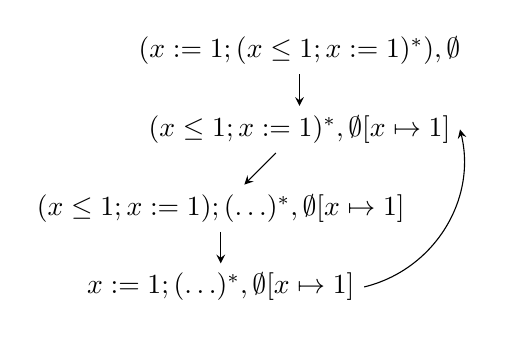
\begin{tikzpicture}[->,>=stealth]
      \node (a) {\(\sem{(x:=1; (x\leq 1; x:=1)^*), \emptyset}\)};
      \node (b) [below of = a] {\(\sem{(x\leq 1; x:=1)^*, \emptyset[x\mapsto 1]}\)};
      \node (c) [below of = b, left of = b] {\(\sem{(x\leq 1; x:=1);(\dots)^*, \emptyset[x\mapsto 1]}\)};
      \node (d) [below of = c] {\(\sem{x:=1;(\dots)^*, \emptyset[x\mapsto 1]}\)};

      \path
      (a) edge (b)
      (b) edge (c)
      (c) edge (d)
      (d.east) edge [bend right=45] (b.east);
    \end{tikzpicture}
    \caption{Execution graph of \((x:=1; (x\leq 1;
      x:=1)^*)\)}\label{fig:exegraphnont}
  \end{figure}
\end{example}


The next step is to prove that a given a finite set of initial states
and a program, if we know that the final invariant is finite, we cound
decide termination:

\begin{lemma}[Finite invariant on finite program]
  Given a finite set of initial states \(X \in 2^\env\), a program
  \(C\in\imp\), ``\(\sem{C}X = Y\) is finite'' is undecidable.
\end{lemma}

\begin{proof}
  Suppose we can decide weather \(\sem{C}X\) (the most precise
  invariant for the program C) is finite. Based on the result we have
  2 options:
  \begin{itemize}
  \item \textbf{The invariant is infinite}: in this case because of
    observation \ref{obs:finite}, we can say that the original program
    does not halt, as it would not terminate in a finite amount of
    steps. Additionally, because of lemma \ref{le:infinitebranch} the
    execution graph of the program contains an infinite branch, which
    is the one responsible for non-termination.
  \item \textbf{The invariant is finite}: This does not give direct
    informations about the termination of the program, because like in
    example \ref{ex:loop} the program can have a finite invariant but
    it might not terminate due to the presence of a cycle in the
    termination graph. However it means that there's no infinite
    branch in the execution graph of \(C\).

    %% dire bene, ci devono essere un numero finito di stati e quindi
    %% posso esplorare il sistema di transizioni
    The initial set of environments is finite, therefore consider
    \(\forall \rho \in X\), the execution graph \(\exec(C, \rho)\): It
    is composed of a finite set of environments, therefore by running
    any cycle-finding algorithm (bfs should do, as in
    \cite{cormen2022introduction}) we have 2 kinds of output:
    \begin{itemize}
    \item there is a cycle, in this case the execution graphs has the
      shape as in figure \ref{fig:cycle}, therefore there's a possible
      execution that never terminates.
      \begin{figure}
        \centering
        \usetikzlibrary{positioning}
        \usetikzlibrary{graphs}
        \begin{tikzpicture}[->,>=stealth]
          \node (start)                {\(\cdot\)};
          \node (bls) [right of=start] {\(\cdot\)};
          \node (cle) [below of=bls]   {\(\dots\)};
          \node (end) [right of=bls]   {\(\cdot\)};

          \path
          (start) edge (bls)
          (bls) edge [bend left] (cle) edge (end)
          (cle) edge [bend left] (bls);
        \end{tikzpicture}
        \caption{example of an execution graph that contains a
          cycle}\label{fig:cycle}
      \end{figure}
    \end{itemize}
  \end{itemize}
\end{proof}
